% !TEX program = xelatex
\documentclass[11pt]{article}

\usepackage{fontspec}
\usepackage{unicode-math}
\setmainfont{Latin Modern Roman}
\setsansfont{Latin Modern Sans}
\setmonofont{Latin Modern Mono}[Scale=0.88]

\usepackage{graphicx}
\graphicspath{{figures/}{../../papers/arxiv-ac/figures/}}
\usepackage{booktabs}
\usepackage{tabularx}
\usepackage{ragged2e}
\usepackage{microtype}
\usepackage{natbib}
\usepackage{listings}

\makeatletter
\def\input@path{{../}}
\makeatother
\usepackage{ac-paper-cards}

\hypersetup{
  pdftitle={Canciones Populares Tocables: La Tradición Oral Encuentra el Teclado del Navegador},
}

% Listing style for notepat song notation
\lstdefinestyle{notepat}{
  basicstyle=\ttfamily\small,
  breaklines=true,
  columns=flexible,
  keepspaces=true,
  showstringspaces=false,
}

\begin{document}

% ============================================================
% TITLE CARD
% ============================================================
\thispagestyle{empty}
\vspace*{\fill}
\begin{center}
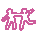
\includegraphics[height=3em]{pals}\par\vspace{0.6em}
{\acbold\fontsize{20pt}{24pt}\selectfont\color{acdark} Canciones Populares}\par
{\acbold\fontsize{20pt}{24pt}\selectfont\color{acdark} Tocables}\par
\vspace{0.3em}
{\aclight\fontsize{10pt}{12pt}\selectfont\color{acpink} La Tradición Oral Encuentra el Teclado del Navegador}\par
\vspace{0.8em}
{\normalsize Jeffrey Alan Scudder}\par
{\small\color{acgray} Aesthetic.Computer}\par
{\small\color{acgray} ORCID: \href{https://orcid.org/0009-0007-4460-4913}{0009-0007-4460-4913}}\par
\vspace{0.3em}
{\small\color{acpurple} \url{https://notepat.com}}\par
\vspace{0.8em}
\rule{0.6\textwidth}{1pt}\par
\vspace{0.4em}
{\small\color{acpink}\textbf{[ borrador de trabajo --- no citar ]}}\par
\vspace{0.3em}
{\footnotesize\color{acgray} Marzo 2026}\par
\end{center}
\vspace*{\fill}

% ============================================================
% ABSTRACT CARD
% ============================================================
\clearpage
\begin{accentcard}
\cardtitle{Resumen}

Las canciones populares evolucionaron para ser tocables sin partitura, memorizables sin instrumentos y bifurcables sin permiso. Estas propiedades---rango tonal limitado, estructura repetitiva, transmisibilidad oral---hacen que las melodías populares sean estructuralmente ideales para un sintetizador de teclado basado en navegador.

\vspace{0.3em}

Este artículo describe la integración de canciones populares tocables en \np{}.com, un instrumento de teclado cromático que asigna las teclas QWERTY a notas musicales. Codificamos melodías populares en un formato ligero \texttt{NOTE:word} que empareja cada altura tonal con su sílaba de la letra, creando un modo de interpretación guiada donde el instrumento enseña la canción una nota a la vez.

\vspace{0.3em}

Examinamos colecciones de melodías populares adecuadas para esta codificación, analizamos por qué las restricciones estructurales de las canciones populares se alinean con las interfaces de teclado-como-instrumento, y argumentamos que el proceso folk---variación, selección, transmisión oral---tiene un análogo digital natural en codificaciones de canciones compartibles por URL y bifurcables.
\end{accentcard}

% ============================================================
% SECTION 1: THE ARGUMENT
% ============================================================
\section{El Argumento}

Las canciones populares son el software de código abierto más antiguo de la humanidad.

No tienen un solo autor. Son mantenidas por una comunidad. Se transmiten oralmente---lo que significa que deben ser lo suficientemente simples para memorizar, lo suficientemente restringidas para reproducir y lo suficientemente flexibles para adaptar. Cada cantante es un colaborador; cada interpretación es una bifurcación.

\vspace{0.3em}

Estas son exactamente las propiedades que hacen que una melodía sea tocable en un teclado QWERTY.

\begin{card}
\cardtitle{¿Por qué canciones populares?}
\begin{itemize}
  \item \textbf{Rango tonal estrecho}: La mayoría de las melodías populares abarcan 1--1,5 octavas~\citep{lomax1968folk}. La cuadrícula de dos octavas de botones de \np{} las cubre en su totalidad.
  \item \textbf{Sesgo pentatónico}: Muchas tradiciones favorecen escalas de 5 notas~\citep{kodaly1971folk}, reduciendo la carga cognitiva de encontrar la siguiente nota.
  \item \textbf{Estructura repetitiva}: Frases de 8 compases que se repiten, patrones de llamada y respuesta, formas de estrofa-estribillo---todo ayuda a la memorización y la reproducción guiada.
  \item \textbf{Sin notas equivocadas}: En las melodías pentatónicas, los tonos adyacentes de la escala son consonantes. El método Orff Schulwerk explota esta misma propiedad con barras de xilófono removibles~\citep{orff1978schulwerk}.
\end{itemize}
\end{card}

% ============================================================
% SECTION 2: THE INSTRUMENT
% ============================================================
\section{El Instrumento}

\np{}.com es un sintetizador cromático basado en navegador construido como una ``pieza'' (programa interactivo) dentro de \ac{}~\citep{scudder2026ac, scudder2026notepat}. Asigna el teclado QWERTY a 24 notas cromáticas a lo largo de dos octavas, con cambio de octava para cubrir todo el rango del piano.

\begin{darkcard}
\textbf{El modo canción} transforma \np{} de un instrumento de interpretación libre en una interfaz de interpretación guiada. Una pista de letras desplazable muestra la sílaba actual; solo la nota correcta está activa; presionarla avanza a la siguiente sílaba. El intérprete no puede cometer un error---solo puede esperar.
\end{darkcard}

Este enfoque de ``ruedas de entrenamiento''---bloquear las notas incorrectas, resaltar la correcta---refleja las pedagogías Orff y Kod\'aly, que restringen el instrumento para adaptarse a la capacidad actual del aprendiz~\citep{kodaly1971folk, orff1978schulwerk}.

% ============================================================
% SECTION 3: THE ENCODING
% ============================================================
\section{La Codificación}

Las canciones en \np{} se codifican como pares \texttt{NOTE:word} separados por espacios:

\notesong{C:Twin- C:-kle G:twin- G:-kle A:lit- A:-tle G:star,\\
F:how F:I E:won- E:-der D:what D:you C:are.}

Cada token es un nombre de nota (\texttt{C}, \texttt{G}, \texttt{A}, \texttt{F\#}, etc.) emparejado con una sílaba de la letra mediante dos puntos. Los guiones indican continuación de sílaba: un guion al final (\texttt{Twin-}) significa que el siguiente token continúa la misma palabra; un guion al inicio (\texttt{-kle}) es la continuación.

\begin{card}
\cardtitle{Propiedades de diseño}
\begin{itemize}
  \item \textbf{Legible por humanos}: Un músico puede leer la codificación directamente a primera vista.
  \item \textbf{Seguro para URL}: Las canciones pueden pasarse como parámetros de URL a \np{}.
  \item \textbf{Bifurcable}: Copiar, editar, compartir---el proceso folk en una cadena de texto.
  \item \textbf{Mínimo}: Sin duración, sin dinámicas, sin tempo. El intérprete controla los tres.
\end{itemize}
\end{card}

La ausencia de información rítmica es deliberada. En la tradición oral, el ritmo pertenece al intérprete, no a la partitura~\citep{lomax1968folk}. La codificación captura \emph{qué} tocar; el intérprete decide \emph{cómo}.

% ============================================================
% SECTION 4: A CATALOG
% ============================================================
\section{Un Catálogo de Melodías Tocables}

Examinamos colecciones de canciones populares de múltiples tradiciones y seleccionamos melodías optimizadas para la cuadrícula de dos octavas de \np{}. Criterios de selección: rango tonal $\leq$\,15 semitonos, escala pentatónica o diatónica simple, y reconocimiento cultural.

\begin{card}
\cardtitle{Pentatónicas (5 notas)}
\begin{tabularx}{\linewidth}{Xll}
\toprule
\textbf{Canción} & \textbf{Origen} & \textbf{Rango} \\
\midrule
Amazing Grace & Americana & P5+oct \\
Auld Lang Syne & Escocesa & oct \\
Arirang & Coreana & oct \\
Sakura & Japonesa & m7 \\
Mo Li Hua & China & oct \\
Swing Low & Espiritual & oct \\
\bottomrule
\end{tabularx}
\end{card}

\begin{card}
\cardtitle{Rango estrecho ($<$ octava)}
\begin{tabularx}{\linewidth}{Xll}
\toprule
\textbf{Canción} & \textbf{Origen} & \textbf{Rango} \\
\midrule
Mary Had a Little Lamb & Americana & P5 \\
Hot Cross Buns & Inglesa & M3 \\
Fr\`ere Jacques & Francesa & M6 \\
London Bridge & Inglesa & P5 \\
Korobeiniki & Rusa & oct \\
\bottomrule
\end{tabularx}
\end{card}

\begin{card}
\cardtitle{Modales y diatónicas}
\begin{tabularx}{\linewidth}{Xll}
\toprule
\textbf{Canción} & \textbf{Origen} & \textbf{Rango} \\
\midrule
Greensleeves & Inglesa & 10.ª \\
Scarborough Fair & Inglesa & oct \\
Danny Boy & Irlandesa & 10.ª \\
Shenandoah & Americana & 10.ª \\
Hava Nagila & Israelí & oct \\
\bottomrule
\end{tabularx}
\end{card}

% ============================================================
% SECTION 5: FOLK PROCESS AS VERSION CONTROL
% ============================================================
\section{El Proceso Folk como Control de Versiones}

El Consejo Internacional de Música Folclórica identificó tres propiedades del proceso folk: \emph{continuidad} (vincular el presente con el pasado), \emph{variación} (impulso creativo de los intérpretes individuales) y \emph{selección} (la comunidad determina qué formas sobreviven)~\citep{karpeles1955definition}.

\begin{accentcard}
Estas se corresponden directamente con el control de versiones de software:

\vspace{0.3em}
\begin{tabularx}{\linewidth}{lX}
\textbf{Continuidad} & \texttt{main} branch \\
\textbf{Variación} & commits, forks \\
\textbf{Selección} & decisiones de merge, adopción \\
\end{tabularx}
\end{accentcard}

Una codificación de canción en \np{} es una URL. Compartir una canción es compartir un enlace. Modificar una canción es editar una cadena de texto y compartir un nuevo enlace. La ``tradición oral'' se convierte en una tradición de URLs---la melodía se transmite no a través de la memoria sino a través del hipertexto.

Esto no es metafórico. La base de datos Essen Associative Code (ESAC), iniciada en 1982, codificó $\sim$8.000 canciones populares europeas y chinas en una notación compatible con computadoras inspirada en el \textit{jianpu} chino~\citep{schaffrath1995esac}. El formato \texttt{NOTE:word} de \np{} es un descendiente directo de esta tradición: codificar melodía como texto para que la computación y la transmisión sean posibles.

% ============================================================
% SECTION 6: COMPUTATIONAL MUSICOLOGY
% ============================================================
\section{Dimensiones Computacionales}

Passmore et al.\ modelaron melodías populares como secuencias en evolución a partir de un ``alfabeto'' de 12 alturas tonales, aplicando métodos de alineamiento de secuencias tomados de la genética molecular a 10.062 melodías japonesas e inglesas~\citep{passmore2023cultural}. Encontraron que los cambios de notas con menor impacto melódico tienen más probabilidad de sobrevivir---una presión selectiva que favorece la simplicidad por la que las canciones populares son conocidas.

\begin{card}
\cardtitle{Por qué esto importa para \np{}}

Si las melodías populares están sujetas a presión de selección evolutiva hacia la simplicidad, entonces están \emph{convergiendo} hacia las propiedades que las hacen tocables en interfaces restringidas. El teclado QWERTY no es un sustituto empobrecido del piano---es una restricción que coincide con la restricción que el proceso folk ya aplica.
\end{card}

El proyecto cantométrico de Lomax codificó 37 aspectos del estilo interpretativo en 5.776 canciones de 1.026 sociedades, encontrando que el estilo interpretativo (no el contenido melódico) era el principal indicador cultural~\citep{lomax1968folk}. Esto respalda la decisión de diseño de \np{} de codificar la altura tonal pero no el ritmo: la variación culturalmente significativa ocurre en \emph{cómo} se interpretan las notas, que es exactamente lo que el intérprete controla.

% ============================================================
% SECTION 7: RELATED INSTRUMENTS
% ============================================================
\section{Instrumentos Relacionados}

\begin{card}
\cardtitle{aQWERTYon}
El Music Experience Design Lab de NYU construyó el aQWERTYon, un instrumento de navegador que asigna las teclas QWERTY a grados de la escala para que no haya ``notas equivocadas''~\citep{hein2017aqwertyon}. \np{} difiere en dos aspectos: utiliza un mapeo \emph{cromático} (las notas equivocadas son posibles y pedagógicamente útiles), y empareja notas con letras de canciones (la canción se enseña a sí misma).
\end{card}

\begin{card}
\cardtitle{ABC Notation}
El estándar de facto para la codificación de música folclórica, ABC notation representa melodía como texto~\citep{walshaw2011abc}. La biblioteca \texttt{abcjs} renderiza ABC como partitura interactiva en navegadores. La codificación de \np{} es más simple---sin duración, sin barras de compás---porque no es un sistema de notación sino un \emph{guion de interpretación}: le dice al intérprete qué presionar, no cómo se ve la música.
\end{card}

\begin{card}
\cardtitle{Tunepal}
Un sistema de recuperación de información musical que conecta a músicos con 13.290 melodías tradicionales irlandesas mediante consulta-por-interpretación~\citep{duggan2009tunepal}. Tunepal encuentra melodías; \np{} las enseña. Son complementarios.
\end{card}

% ============================================================
% SECTION 8: THE BARE-METAL FOLK INSTRUMENT
% ============================================================
\section{El Instrumento Folk sobre Hardware Puro}

\np{} no solo se ejecuta en navegadores sino sobre hardware puro---un port de 987 líneas en QuickJS que arranca como PID~1 en AC Native OS~\citep{scudder2026os}. Un portátil ejecutando \np{} sobre hardware puro es, en sentido literal, un instrumento folk: un dispositivo de propósito único para tocar canciones, sin sistema operativo, sin escritorio, sin distracciones.

\begin{accentcard}
La convergencia es total: canciones populares, diseñadas para ser tocadas en el instrumento más simple disponible, ejecutándose en la computadora más simple posible---un kernel Linux, un framebuffer y un teclado.
\end{accentcard}

% ============================================================
% SECTION 9: FUTURE WORK
% ============================================================
\section{Trabajo Futuro}

\begin{card}
\begin{itemize}
  \item \textbf{Codificación colaborativa}: Un repositorio público de codificaciones \texttt{NOTE:word}, enviadas como URLs, versionadas como las canciones populares mismas.
  \item \textbf{Colecciones interculturales}: Codificar melodías de los archivos Essen, Roud y Lomax en formato \np{}, con permiso y atribución.
  \item \textbf{Dificultad adaptativa}: Expandir el rango tonal a medida que el intérprete domina canciones más simples---una progresión tipo Kod\'aly a través del repertorio folclórico.
  \item \textbf{Sesiones folk multijugador}: Dos intérpretes de \np{} en la misma canción, uno tocando la melodía, otro la armonía---una \textit{session} digital en el sentido tradicional irlandés.
  \item \textbf{Grabación y compartición}: Capturar una interpretación como audio, emparejarla con la URL de codificación y publicarla---una tradición oral con constancia.
\end{itemize}
\end{card}

% ============================================================
% CONCLUSION CARD
% ============================================================
\section{Conclusión}

Las canciones populares sobrevivieron siglos sin notación, sin grabación, sin instrumentos. Sobrevivieron porque eran lo suficientemente simples para recordar, lo suficientemente flexibles para adaptar y lo suficientemente valiosas para compartir.

Un teclado de navegador que enseña estas canciones una nota a la vez no es una desviación de la tradición folclórica. \emph{Es} la tradición folclórica---adaptada, una vez más, al instrumento que se tiene a mano.

\vspace{0.5em}
\noindent\textbf{ORCID:} \href{https://orcid.org/0009-0007-4460-4913}{0009-0007-4460-4913}

\bibliographystyle{plainnat}
\bibliography{references}

\end{document}
